\documentclass[../main.tex]{subfiles}
\begin{document}
\chapter{O CONJUNTO DOS NÚMEROS NATURAIS E OS AXIOMAS DE PEANO}
Neste capítulo apresentaremos os números naturais. Primeiro será apresentada brevemente parte histórica e sua importância, após isso, enunciaremos os axiomas. Depois definiremos uma adição, uma multiplicação e uma relação de ordem, bem como listaremos algumas propriedades básicas e faremos sua demonstração. As referências básicas desse capítulo são DOMINGUES e FERREIRA.

\section{Um pouco de história}
Aprendemos na escola, que os seres humanos começaram a trabalhar com números muito antigamente. Os números eram utilizados para contar. Ao longo do tempo, esse manuseio dos números foi ficando mais complexo até chegar na crise da matemática no século XIX e XX. Essa crise levou os matemáticos a buscarem a formalização da matemática.

Os números naturais foram os que mais resistiram ao tempo na sua formalização. Uma tentativa que na época não ficou muito difundida foi, em 1888 por Dedekind, a formalização dos naturais. No entando, apenas no ano seguinte, pelo italiano Giuseppe Peano, a formalização ficou amplamente difundida. O trabalho de Peano utilizou o de Dedekind como base. CITAR

Peano em seu 'Arithmetices Principia, Nova Methodo Exposita' fundamentou a sua aritmética com 9 axiomas, como extraído abaixo e com 3 conceitos primitivos.
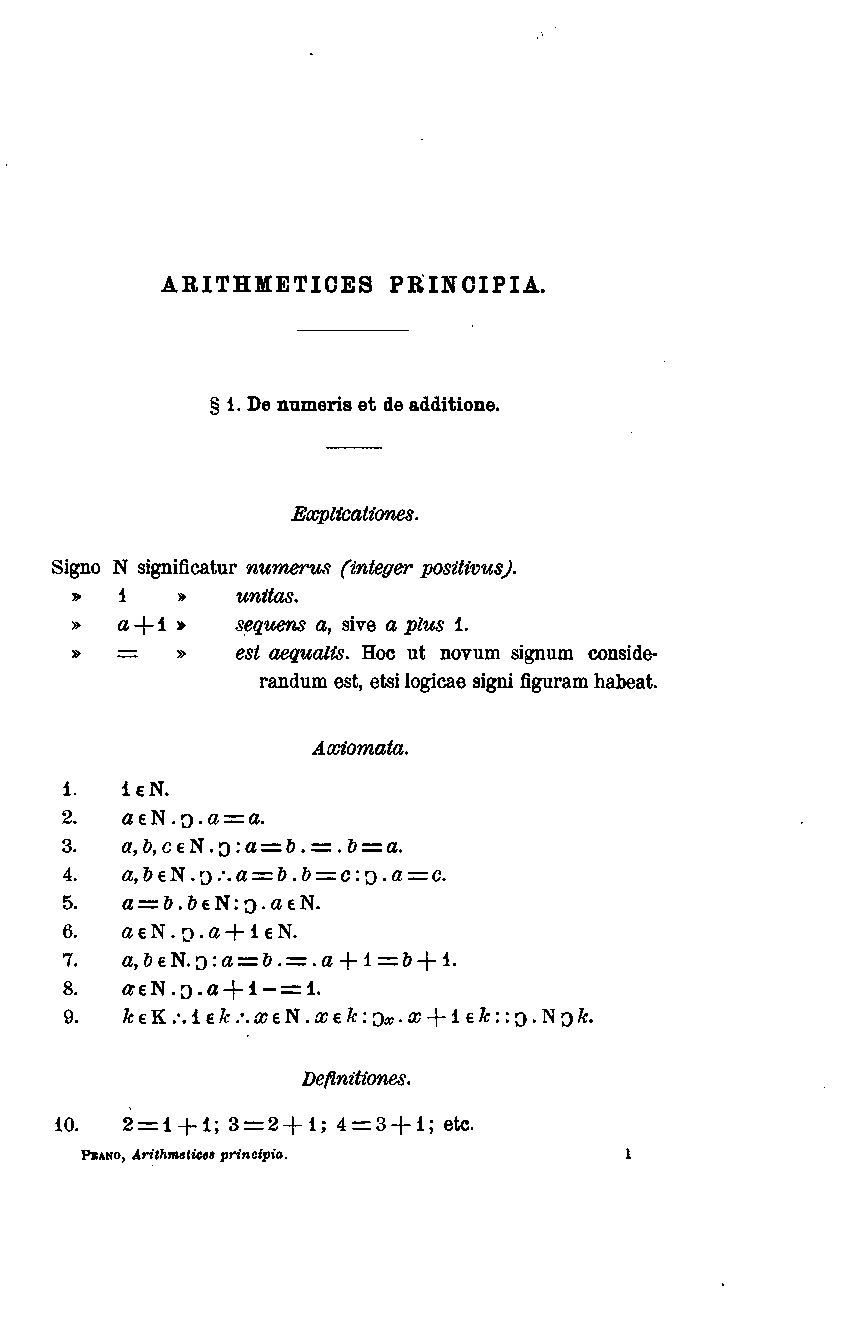
\includepdf{../include/peano_axioms_original.pdf}
CITAR

"Ao cirar um jogo, é importante que suas regras sejam suficientes e consistentes. Por \emph{suficiente} queremos dizer que as regras devem estabelecer o que é permitido fazer em qualquer situação que possa viar a ocorrer no desenrolar de uma partida do jogo. Por \emph{consistente} queremos dizer que as regras não devem contradizer-se, ou sua aplicação levar a situações contraditórias." CITAR.

Para nós, as peças do jogo serão o conceito de um, o conceito de número natural, e o conceito da relação sucessor. As regras do jogo, naturalmente serão os axiomas que relacionarão esses 3 conceitos primitivos. Nessa analogia, as peças não são muito importantes.

\section{Axiomas}
O nosso estudo dos números naturais será iniciado pela sua apresentação em 3 conceitos primitivos, como os de Peano, e 5 axiomas (ao invés de 9), que são:

\begin{axi}\label{axi-existe-n-s}
    Existe um conjunto de exatamente todos os números naturais, que será denotado por $\N$, e existe uma função $s: \N \rightarrow \N$, que é a relação "sucessor". 
    % TODO \footnote{O leitor poderia perguntar, como podemos fazer um produto cartesiano de conjuntos que não conhecemos?}
\end{axi} % TODO Não teria que especificar que é o mesmo 's' em todos os axiomas?
\begin{axi}\label{axi-um-natural}
    Um é um número natural, isto é, $1 \in \N$.
\end{axi}
\begin{axi}\label{axi-um-nao-sucessor}
    Um não é sucessor de nenhum número, isto é, $1 \not \in Im(s)$ ou ainda, $\not \exists x \in \N : s(x) = 1$.
\end{axi}
\begin{axi}\label{axi-s-injetora}
    $s$ é injetora, isto é, $s(x) = s(y) \implies x = y$ \footnote{Vale notar a contra-positiva que estabelece, nesse caso: $x \neq y \implies s(x) \neq s(y)$}.
\end{axi}
\begin{axi}\label{axi-ind-finita}
    Se $\S$ é um subconjunto de $\N$, caso $1 \in \S$ e se para todo $k$ em $\S\ s(k)$ também esteja em $\S$, então $\S = \N$, isso é o mesmo que colocar:
     $\S \subseteq \N \land 1 \in S \land ( k \in \S \implies s(k) \in \S) \implies \S = \N$.
\end{axi}
Este último axioma é chamado de axioma da indução finita.

Conforme os axiomas aprsentados, deve ser notado que o conjunto \N (na nossa axiomatização) não tem o $0$ (zero) que é, usualmente, o neutro da soma em \N. O intuito de construir a partir do $1$ é pela questão que às vezes surge em diversas situações: "$0$ é um número natural?". Em diversos locais, dizem que pode ser e pode não ser. É dito que fica a critério de conveniência, embora para nós, seja 'inconveniente' perder o neutro da soma (que aparecerá sua primeira vez em \Z). 

Justificamos essa escolha pois essa dificuldade na ausência do zero terá algumas implicações, que poderão ser observadas na nossa construção. Além disso, a bibliografia principal trata o zero como um número natural, então a construção será necessariamente com essas adaptações, o que na visão do autor, é algo positivo para o desenvolvimento do trabalho, mas o resultado final em certo ponto de vista fica prejudicado, pois fica mais "remendado".

Observemos também que o próprio Peano começou originalmente pelo $1$ e somente depois colocou o $0$ como o primeiro número natural.

Para comerçarmos nosso desenvolvimento, podemos notar que o axioma \ref{axi-um-natural} garante $\N \neq \emptyset $. Além dele, como $1 \in \N$ e pelo axioma \ref{axi-existe-n-s} temos que $s(s(1)) \in \N$. Analogamente, $s(s(s(1))) \in \N$.

Em seguida apresentamos um lema que será necessário para ampliação de nosso ferramental inicial.
\begin{lema}{Nenhum número natural é seu próprio sucessor}\label{n-dif-sucessor}
    $x \in \N \implies x \neq s(x) $.
\end{lema}
\begin{dem}
    Faremos por indução. Seja $\S = \{x \in \N : x \neq s(x) \}$
    Os axiomas \ref{axi-um-natural} e \ref{axi-um-nao-sucessor} garantem que $1 \in \S$.\\
    Supondo que $\exists k \in \S : k \neq s(k)$, queremos provar que o sucessor de $k$ é diferente do sucessor do sucessor de $k$, isto é, $s(k) \neq s(s(k))$. Como $k \neq s(k)$ e $s$ é injetora pelo axioma \ref{axi-s-injetora}, concluímos que $s(k) \neq s(s(k))$.
\end{dem}
\begin{teo}\label{suc-unico}
    Todo número natural, exceto o $1$ é sucessor de algum outro número natural, que é único, isto é, $\forall x (x \in \N \land x \neq 1 \implies \exists! y : s(y) = x)$.
\end{teo}
\begin{dem}
    A prova é feita por indução. Seja $\S = \{x \in \N : x \neq 1 \implies (\exists!y \in \N : s(y) = x)\}$.\\
    sabemos que $1 \in \S$ porque $x = 1$ torna o antecedente falso, onde podemos concluir qualquer coisa. Suponhamos que existe um $k$ em \S, queremos mostrar que $s(k) \in \S$. \\
    É imediato que $s(k) \in \S$ pois, se $k \in \S$, para o sucessor $s(k)$ existe um número $k$ tal que $\underbrace{s(k)}_{\text{Da regra de } \S} = \underbrace{s(k)}_{\text{Axioma }\ref{axi-ind-finita}}$.\\
    A unicidade de $y$ também é imediata, pois $s(a) = s(b) = k \implies a = b$ pela injetividade de $s$ axioma \ref{axi-s-injetora}.
\end{dem}
\begin{obs}
    Diremos que o número $y$ é antecessor de $x = s(y)$. Além disso vale notar que $s$ conforme definida no axioma \ref{axi-existe-n-s} não é sobrejetora somente pelo fato de o contradomínio ser \N. Mas se considerarmos o caso restrito para $\N \setminus \{1\}$ 
    teremos que $s$ é uma \emph{bijeção}.
\end{obs}


%%% ADICAO %%%


\section{A adição}
A adição em \N é a que mais intuitivamente está relacionada com a contagem e união de coisas discretas.
\begin{defi}{Adição}\label{def-adicao-N}
Sejam $x, y \in \N$. A adição entre $x$ e $y$, denotada por $x + y$ é definida com as seguintes condições: 
    \begin{enumerate}[label=(\roman*)]
        \item $x + 1 = s(x)$;
        \item $x + s(y) = s(x+y)$.
    \end{enumerate}
\end{defi}
Às vezes poderemos fazer referência à operação de adição com o nome de soma.
\begin{lema}\label{soma-n-um-comut}
    O $1$ comuta com qualquer número na soma, isto é,$ \forall x, x + 1 = 1 + x$
\end{lema}
%        Seja $\S = \{ x \in \N : \}$
\begin{dem}
    Seja $\S = \{ x \in \N : x + 1 = 1 + x\}$. O $1$ está em \S pois $1 + 1 = 1 + 1$.
    sabendo que existe um $k$ em \S, queremos provar que $s(k)$ também está em \S. Como
    $s(k) + 1 = s(s(k)) = s(k+1) = s(1+k) = 1 + s(k)$. Portanto $s(k)$ também está em \S sempre que $k$ também está, o que pelo princípio de indução \S = \N.
\end{dem} \\

Abaixo veremos algumas propriedades básicas sobre a adição no conjunto \N.
\begin{prop}{Sejam $a, b, c, d \in \N$ valem:}\label{soma-props}
    \begin{enumerate}[label=(\roman*)]
    	\item Associativa: $(a + b) + c = a + (b + c)$;
    	\item Comutativa: $a + b =  b + a$;
        \item Fechamento: $a + b \in \N$;
        \item Lei do cancelamento: $a + c = b + c \implies a = b$;
        \item $a + b \neq a$;
    	\item Inexistência de neutro: $\not\exists e \in \N : \forall a, a + e = e + a = a$.
    \end{enumerate}
\end{prop}

\begin{dem}
    \begin{enumerate}[label=(\roman*)]
        \item Associativa: \\
             Seja $\S = \{ x \in \N : (a + b) + x = a + (b + x) \}$. Para o $1$ temos então
             $(a + b) + 1 = s(a + b) = a + s(b) = a + (b + 1)$, o que mostra que o $1$ está em \S. 
             Mostraremos que $k \in \S \implies s(k) \in \S$, pois:
             $(a + b) + s(k) = s( (a + b) + k) = s(a + (b + k)) = a + s(b + k) = a + (b + s(k))$, o que, pelo princípio de indução \S = \N.
        
            Com isso tomamos a liberdade natural de omitir os parênteses na soma.
       
        \item Comutativa: \\
            Consideremos o conjunto $\S = \{ x \in \N : a + x = x + a\}$. O $1 \in \S$ pois 
            $a + 1 = 1 + a$ conforme o lema \ref{soma-n-um-comut}.
            Provemos então que se $k \in \S$ então $s(k) \in \S$, pois 
            $a + s(k) = s(a + k) = s(k + a) = k + s(a) = k + a + 1 = k + 1 + a = s(k) + a$
    
        \item Fechamento: \\
            Seja $\S = \{ x \in \N : a + x \in \N \}$. Obviamente o $1$ está em \S. Suponhamos então que existe $k \in \S$, queremos saber se isso garante que $s(k) \in \S$. Temos então que $a + k \in \N$, já para $a + s(k) = a + k + 1 = (a + k) + 1 = s(a + k) \in \S$ pelo axioma \ref{axi-existe-n-s} a função tem domínio e contradomínio \N.
    
    
        \item Lei do cancelamento: \\
            Seja $\S = \{ x \in \N : x + b = x + c \implies b = c \}$, vamos provar que \S = \N. Obviamente o $1$ está em \S pois $1 + b = 1 + c \iff b + 1 = c + 1$ e pelo axioma da injetividade, se dois elementos tem sucessores iguais, eles próprios são iguais. Agora consideremos se vale que $(k + b = k + c \implies b = c) \implies (s(k) + b = s(k) + c \implies b = c)$. \\
            $s(k) + b = s(k) + c \iff (k + b) + 1 = (k + c) + 1$, o que pelo mesmo motivo anterior, concluímos que $k + b = k + c$, e pela nossa hipótese concluímos que $b = c$.
    
        \item $a + b \neq a$;\\
            Consideremos quatro casos:
            \begin{enumerate}[label=(\arabic*)]
            \item $a=1 \land b=1$ \\
                Temos $a+b=a \iff 1+1=1 \absurd$. \\
            \item $a=s(x) \land b=1$ \\
                Temos $a+b=a \iff s(x) + 1 = s(x) \iff s(s(x)) = s(x) \absurd$. \\
            \item $a=1 \land b=s(y)$ \\
                Temos $a+b=a \iff 1+ s(y) = 1 \iff s(1+y) = 1 \absurd$. \\
            \item $a=s(x) \land b=s(y)$ \\
                Temos $a+b=a \iff s(x) + s(y) = s(x) \iff x + 1 + y + 1 = x + 1 \iff s(1 + y) = 1 \absurd$.
            \end{enumerate}
    
        \item Inexistência de neutro: \\
            Como consequência da demonstração anterior, temos que não existe neutro na adição, isto é, $a + e = e + a = a$.
    \end{enumerate}
\end{dem}
 
Podemos observar que como não existe neutro, não poderemos aplicar descuidadamente as outras propriedades, por exemplo: não poderíamos ter provado que $a \neq a+ 1 $ usando a lei do corte e supondo que fossem iguais, assim: $a = a+ 1 \implies 0 = 1$, porque isso não faz sentido no nosso desenvolvimento.

%%% MULTIPLICACAO %%%
A multiplicação toma seu lugar como uma operação de redução da soma. É verdade que sem a notação do sistema posicional, o que nos possibilitaria interpretar $10 = s(9)$, dizer que a multiplicação é um resumo ou simplificação da computação da soma não faz muito sentido. Não faremos o uso do sistema posicional aqui em \N. 


\section{A multiplicação}
\begin{defi}{Multiplicação}\label{def-multiplicacao-N}
    Sejam $x, y \in \N$. A multiplicação entre $x$ e $y$, denotada por $x \cdot y$ é definida com as seguintes condições: 
	\begin{enumerate}[label=(\roman*)]
		\item $x \cdot 1 = x$;
		\item $x \cdot s(y) = x + x \cdot y$.
	\end{enumerate}
\end{defi}
\begin{obs}
	Com o intuito de omitir parênteses que seriam usados demais de outro modo, estebeleceremos a seguinte convenção: 
	\begin{center}
    	$x + y \cdot z \defeq x + (y \cdot z)$ \footnote{$\defeq$ é o símbolo que representa que o que está à esquerda é por definição igual ao que está à direita} \\
    	$x \cdot y + z \defeq (x \cdot y) + z$; \\
    	$x \cdot y \defeq xy$	    
	\end{center}

\end{obs}

Enunciaremos abaixo algumas propriedades da multiplicação.
\begin{prop}{Sejam $a, b, c, d \in \N$ valem:}
    \begin{enumerate}[label=(\roman*)]
        \item Elemento neutro: $\exists! e \in \N : a \cdot e = e \cdot a = a$; \footnote{Se for observada a definição de multiplicação, esse número pode ser o $1$}.
        \item Distributiva à esquerda: $a \cdot (b + c) = ab + ac$;
        \item Associativa: $(a \cdot b) \cdot c = a \cdot (b \cdot c)$;
        \item Distributiva à direita: $(a + b) \cdot c = ac + bc$;
        \item Comutativa: $a \cdot b = b \cdot a$;
        \item Lei do cancelamento: $a \cdot b = a \cdot c \implies b = c$;
        \item $a \cdot b = 1 \implies a = b = 1$.
    \end{enumerate}
\end{prop}
% Seja $\S = \{ x \in \N : \}$
\begin{dem}
    \begin{enumerate}[label=(\roman*)]
        \item Elemento neutro: \\
            Seja $\S = \{ x \in \N : 1 \cdot x = x \cdot 1 \}$. O $1$ está em \S pois $1 \cdot 1 = 1 \cdot 1$. Supondo que $k \in \S$ podemos concluir que $s(k) \in \S$?
            Temos $1 \cdot s(k) = 1 + 1 \cdot k = 1 + k \cdot 1 = 1 + k = s(k) = s(k) \cdot 1$. \\ Além disso, sejam $e_1, e_2$ dois elementos neutros. Então $e_1 = e_1 \cdot e_2 = e_2 \implies e_1 = e_2$, portanto o neutro é único. Além disso a definição de multiplicação nos diz que é o $1$ quem é o neutro. 
            
        \item Distributiva à esquerda: \\
            Seja $\S = \{ x \in \N : a(b+x) = ab+ax\}$. O $1$ está em \S pois $a(b+1) = a(s(b)) = a + ab = a \cdot 1 + ab$. Supondo que existe um $k \in \S$, queremos concluir que $s(k)$ também está em \S.
            Como $a(b+s(k)) = a(s(b+k)) = a + (a(b+k)) = a+(ab+ak) = ab + a + ak = ab+a \cdot s(k) $. Pelo axioma \ref{axi-ind-finita} tem-se que \S = \N.
        \item Associativa:  \\
            Seja $\S = \{ x \in \N : a(bx) = (ab)x \}$. Sabemos que o $1$ está em \S pois $a (b \cdot 1) = a(b) = ab = (ab)\cdot 1$.
            Agora suponhamos que exista um $k \in \S$, consideremos $s(k)$, para ver se ele está ou não em \S. Temos
            $a(b \cdot s(k)) = a(b + bk) = ab + abk = (ab) \cdot s(k)$, o que pelo axioma \ref{axi-ind-finita} tem-se que \S = \N. 
            
        \item Distributiva à direita: 
            Seja $\S = \{ x \in \N : (a+b)x = ax+bx\}$. Temos que o $1 \in \S$ pois $(a+b)1 = a+b = a \cdot 1+b \cdot 1$. Provemos que se $k \in \S$ temos que $s(k) \in \S$. Consideremos então: $(a+b)s(k)=(a+b)(k+1) = (a+b)k + (a+b) \cdot 1 = ak + bk + a + b = a+ak + b + bk = a\cdot s(k) + b \cdot s(k)$. Pelo axioma \ref{axi-ind-finita} tem-se que \S = \N.
            
        \item Comutativa: \\
            Seja $\S = \{ x \in \N : ax = xa \}$. Com certeza o $1$ está em \S, porque $1$ é o neutro da multiplicação. Agora vejamos se $k \in \S$ acarreta que $s(k) \in \S$. Temos então: $a \cdot s(k) = a (k+1) = ak + a = 1 \cdot a + ka = (1+k)a = s(k) \cdot a$. Pelo axioma \ref{axi-ind-finita} tem-se que \S = \N.
            
        \item Lei do cancelamento: \\
            Seja $\S = \{ x \in \N : xb = xc \implies b = c\}$. O $1$ está em \S pois $1b = 1c \implies b = c$. Provemos que $k\in \S \implies s(k) \in \S$. Temos que $s(k) \cdot b = s(k) \cdot c \iff b + bk = c + ck \iff b = c$. Pelo axioma \ref{axi-ind-finita} tem-se que \S = \N.
        \item $a \cdot b = 1 \implies a = b = 1$.
            Consideremos que o $a$ ou o $b$ podem ser igual (ou iguais) a $1$.
            Sem perda de generalidade, seja $a = 1$. Temos que $1 \cdot b = 1 \implies b = 1$ pois $1$ é o elemento neutro. Portanto se algum $a$ ou se $b$ forem iguais a $1$, obrigatoriamente o outro deverá ser, para que a igualdade ocorra.
            Consideremos um último caso, se $a \neq 1 \land b \neq 1$. Então existem $x$ e $y$ naturais tais que $a = s(x)$ e $b = s(y)$.
            Assim, $ab=1 \iff (x+1) (y+1) = 1 \implies 1 + y + 1 + x = 1 \implies s(y + 1 + x) = 1$, o que obviamente não pode ocorrer de acordo com o axioma \ref{axi-um-nao-sucessor}.
    \end{enumerate}
\end{dem}
% Seja $\S = \{ x \in \N : \}$

Nesse desenvolvimento, as propriedades ficaram semelhantes à como seria se fosse incluído o $0$. As propriedades associativa e comutativa já eram presentes na soma. Agora no produto, temos um elemento neutro que não há para a soma, além da distributiva que pode ser aplicada com soma e produto.
Na nossa lei do cancelamento, não precisamos especificar que o termo a ser cancelado é diferente de zero.

%%% A RELACAO DE ORDEM %%%

Até agora dispomos de uma soma e um produto em \N, mas isso ainda não nos possibilita comparar dois elementos de \N. Numa situação simplificada poderíamos legitimamente perguntar se a qunatidade $x$ ou quantidade $y$ é maior ou tem mais. Para essas perguntas, podemos utilizar uma relação de ordem.

Uma relação de ordem em um conjunto em geral não precisa ser única, embora para os fins deste trabalho, as relações de odem em todos os conjuntos que definiremos será a relação de ordem usual, o que poderemos chamar de "a" relação de ordem, ao invés de "uma" relação de ordem.

\section{A relação de ordem}
\begin{defi}\label{def-relOrdem-N}
Sejam $x, y \in \N$. Definiremos a relação $\leq$ entre $x$ e $y$, denotado por $x \leq y$, e diremos que $x$ se relaciona com $y$ através de '$\leq$' quando $x = y \lor x + n = y, n \in \N$.
\end{defi}
\begin{obs}
    Deve ser notado que quando $x \leq y$ uma e apenas uma das seguintes situações pode ocorrer $x = y$ ou $x + n = y, n \in \N$. Isso é devido à propriedade \ref{soma-props}
\end{obs}
\begin{defi}
    Vamos usar a relação $<$ entre $x$ e $y$ dessa forma: $x < y$, para dizer que $x \leq y$ mas $x \neq y$, o que é devido à observação anterior. 
\end{defi}
\begin{prop}{Sejam $a, b, c, d \in \N$ valem:}
    \begin{enumerate}[label=(\roman*)]
        \item Reflexiva: $a \leq a$;
        \item Antissimétrica: $a \leq b \land b \leq a \implies a = b$;
        \item Transitiva: $a \leq b \land b \leq c \implies a \leq c$;
        \item Totalidade: $a \leq b \lor b \leq a$;
        \item Compatível com adição: $a \leq b \iff a + c \leq b + c$;
        \item Compatível com multiplicação: $a \leq b \iff ac \leq bc$.
    \end{enumerate}
\end{prop}
\begin{dem}
    \begin{enumerate}[label=(\roman*)]
        \item Reflexiva: \\
            É imediato que $a = a \implies a \leq a$.
        \item Antissimétrica: \\
            Se $a=b$ não há nada a provar. Consideremos que sejam diferentes.
            Então $a \leq b \iff b = a + n$ e também, como $b \leq a \iff a = b + m$, substituindo, temos $b = (b+m) + n \implies b = b+r$ para algum $r$ natural, o que não pode ocorrer. % como demonstrado no item XXX etc.
        \item
            Vamos considerar 4 casos:
            \begin{enumerate}[label=(\arabic*)]
                \item $a = b = c$ \\
                    Temos $a = c \implies a \leq c$\\
                \item $a = b < c$ \\
                    Temos $ b + n = c \implies a + n = c\implies a \leq c$\\
                \item $a < b = c$ \\
                    Temos $a + n = b = c \implies a \leq c$\\
                \item $a < b < c$ \\
                    Temos $a + m = b \land b + n = c \implies ( a + m ) + n = c \implies a \leq c$
            \end{enumerate}
        \item Totalidade:
        TODO
        \item Compatível com adição: \\
        Seja $a \leq b$. Se $a = b$ teremos que $a+c = b+c$ porque a adição é uma função! 
        Consideremos agora $a < b$. Então $b = a + m \implies b+c = a+m+c \implies a+c < b+c$.
        \item Compatível com multiplicação: \\
        É análogo ao caso da compatibilidade com a adição.
     \end{enumerate}
\end{dem}

Essa é uma relação de ordem pois tem as propriedades $i, ii$ e $iii$.

%\begin{teo}{Princípio do menor elemento}
%...
%\end{teo}
%\begin{teo}{Primeiro princípio de indução}
%...
%\end{teo}
\end{document}